

\[
p = -\lambda {\bm \nabla}\cdot {\bm v}
\]

$q_1$ is smoothed pressure obtained with the  center-to-node approach.

$q_2$ is recovered pressure obtained with \cite{zina82}.

All three fulfill the zero average condition: $\int p d\Omega = 0$.

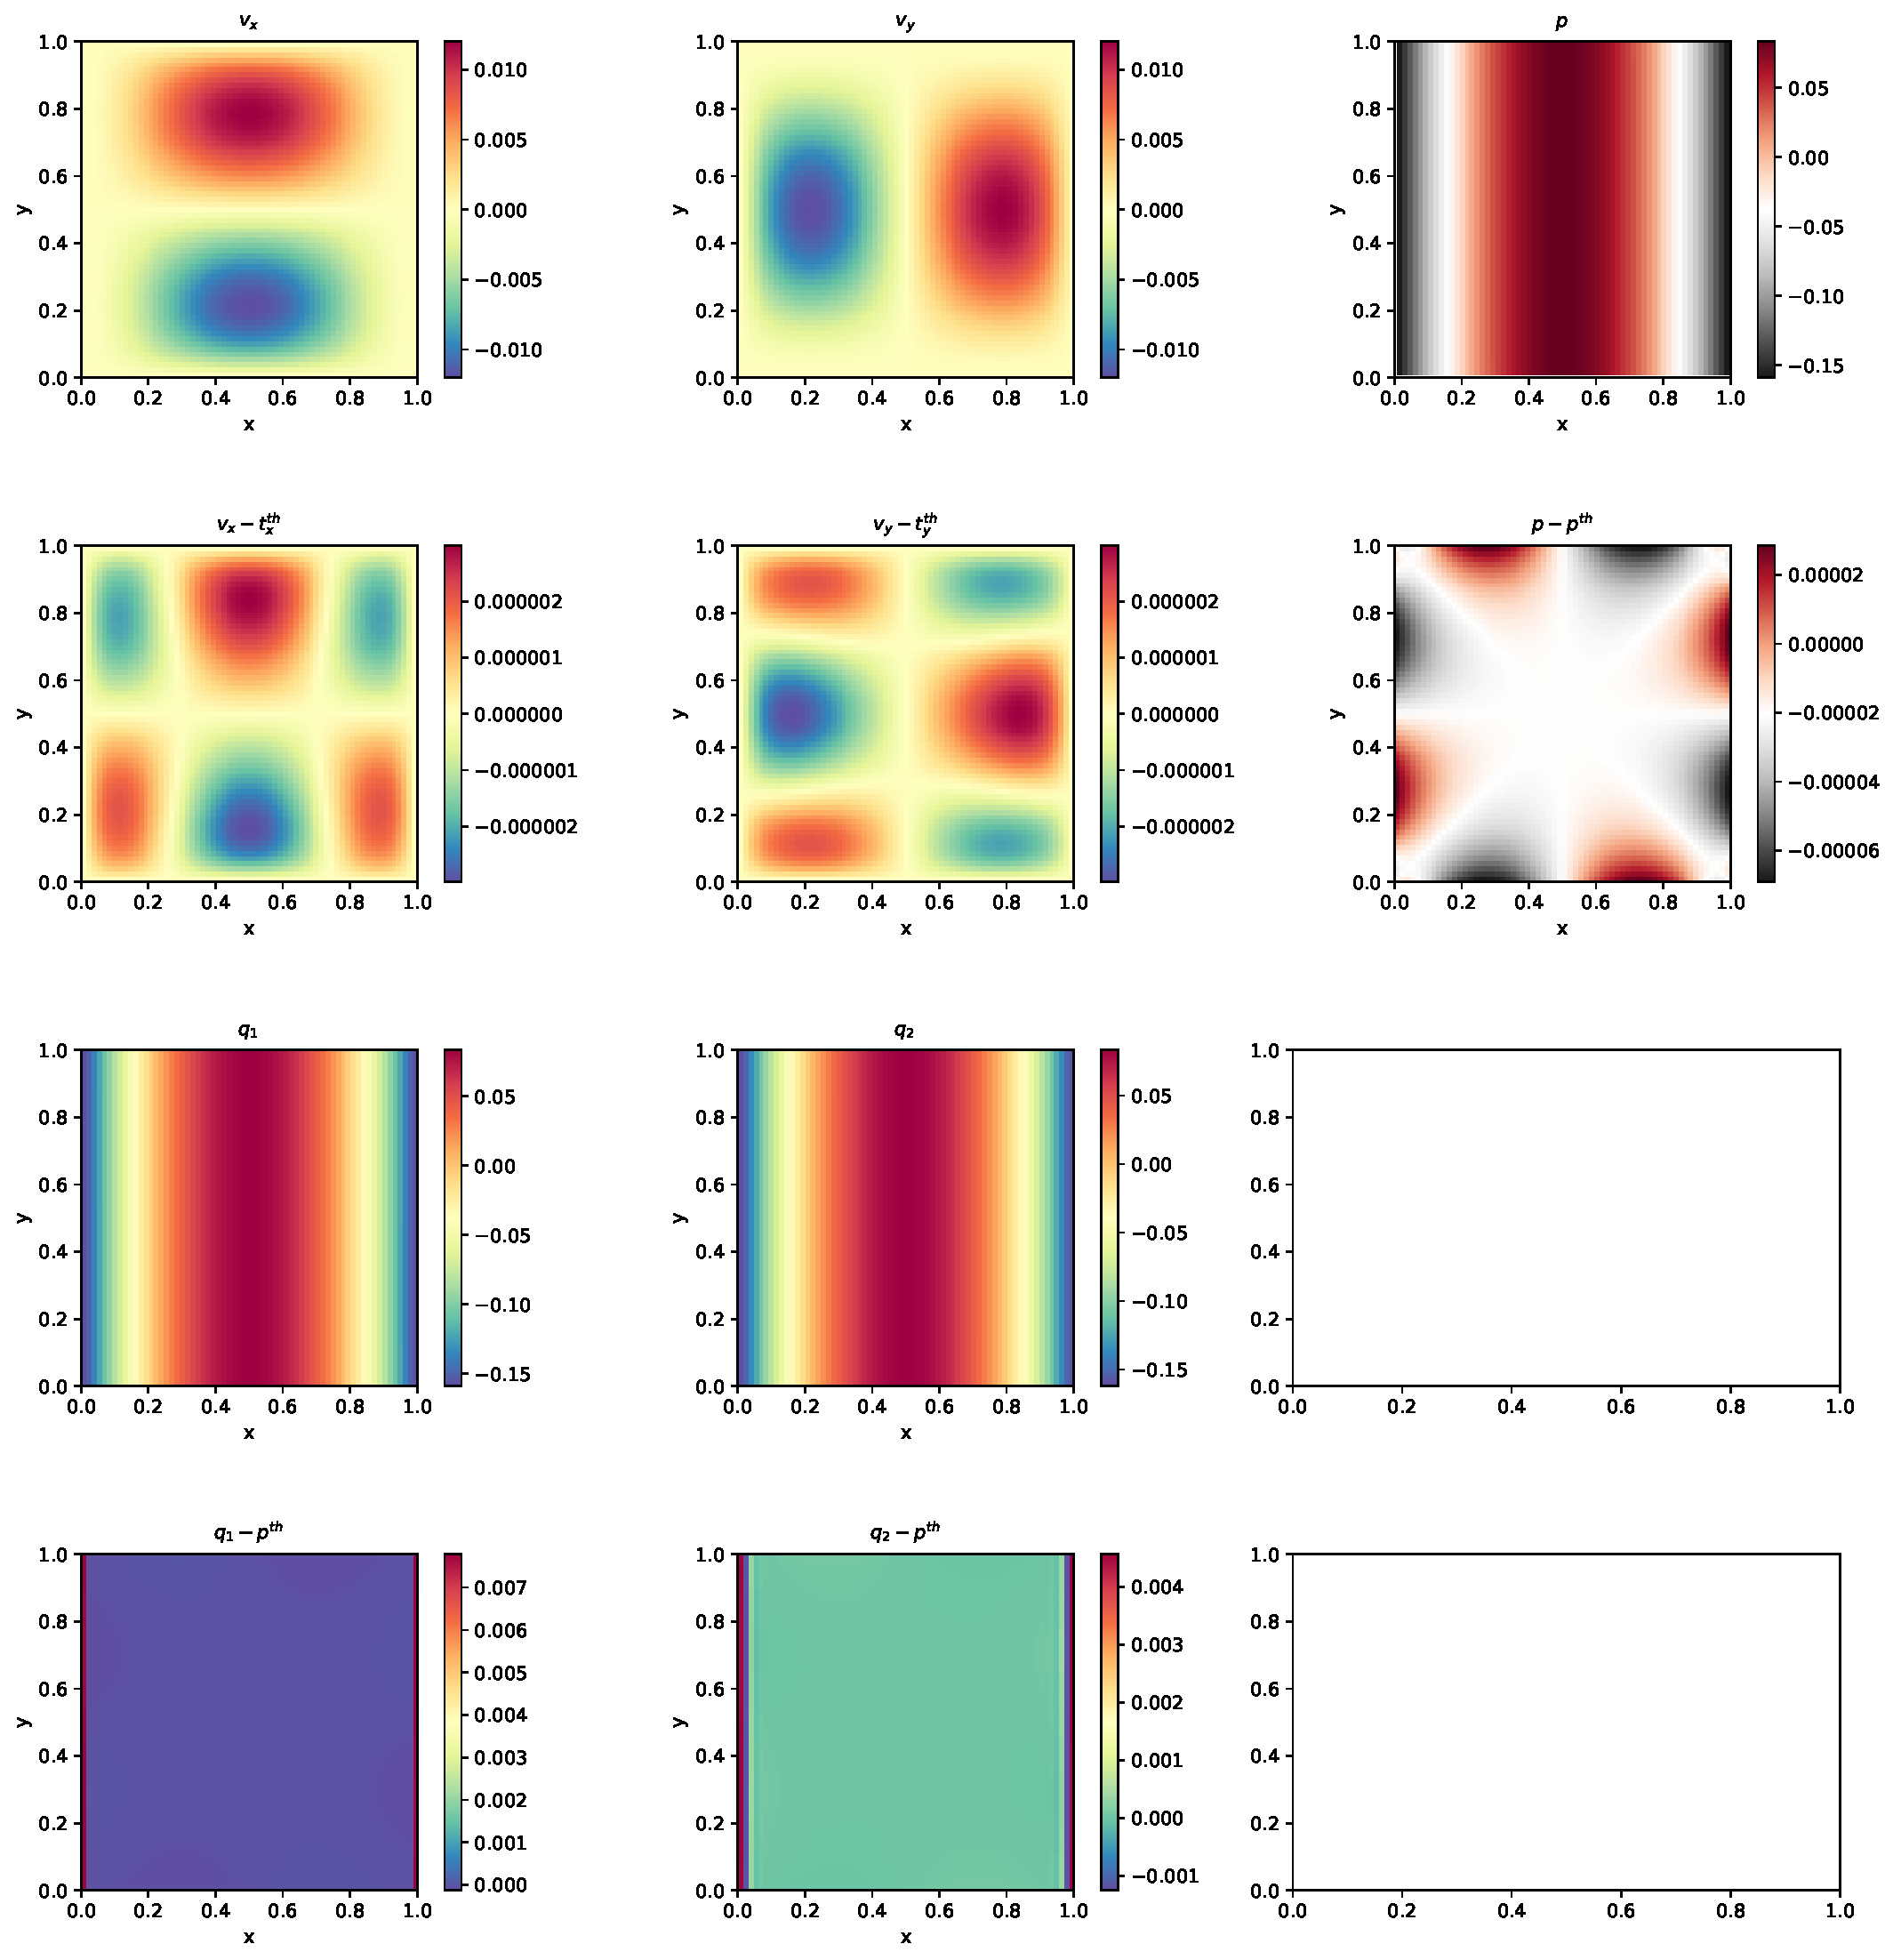
\includegraphics[width=15cm]{python_codes/fieldstone_consistent_pressure_recovery/solution}

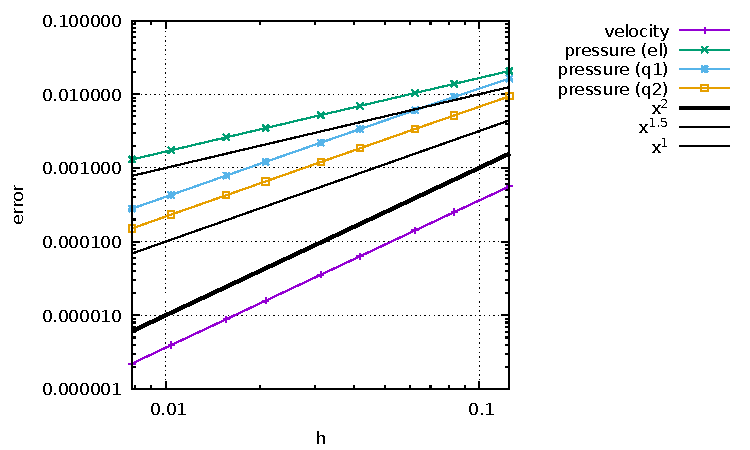
\includegraphics[width=8cm]{python_codes/fieldstone_consistent_pressure_recovery/errors}

In terms of pressure error, $q_2$ is better than $q_1$ which is better than elemental.

QUESTION: why are the averages exactly zero ?!

TODO: 
\begin{itemize}
\item add randomness to internal node positions.
\item look at elefant algorithms
\end{itemize}
